%%%%%%%%%%%%%%%%%%%%%%%%%%%%%%%%%%%%%%%%%
% a0poster Landscape Poster
% LaTeX Template
% Version 1.0 (22/06/13)
%
% The a0poster class was created by:
% Gerlinde Kettl and Matthias Weiser (tex@kettl.de)
% 
% This template has been downloaded from:
% http://www.LaTeXTemplates.com
%
% License:
% CC BY-NC-SA 3.0 (http://creativecommons.org/licenses/by-nc-sa/3.0/)
%
%%%%%%%%%%%%%%%%%%%%%%%%%%%%%%%%%%%%%%%%%

%----------------------------------------------------------------------------------------
%	PACKAGES AND OTHER DOCUMENT CONFIGURATIONS
%----------------------------------------------------------------------------------------

\documentclass[a0,landscape]{a0poster}

\usepackage{multicol} % This is so we can have multiple columns of text side-by-side
\columnsep=100pt % This is the amount of white space between the columns in the poster
\columnseprule=3pt % This is the thickness of the black line between the columns in the poster

\usepackage[svgnames]{xcolor} % Specify colors by their 'svgnames', for a full list of all colors available see here: http://www.latextemplates.com/svgnames-colors

\usepackage{times} % Use the times font
%\usepackage{palatino} % Uncomment to use the Palatino font

\usepackage{graphicx} % Required for including images
\graphicspath{{images/}} % Location of the graphics files
\usepackage{booktabs} % Top and bottom rules for table
\usepackage[font=small,labelfont=bf]{caption} % Required for specifying captions to tables and figures
\usepackage{amsfonts, amsmath, amsthm, amssymb} % For math fonts, symbols and environments
\usepackage{wrapfig} % Allows wrapping text around tables and figures
\usepackage{graphicx} % Allows including images
\usepackage{booktabs} % Allows the use of \toprule, \midrule and \bottomrule in tables
%\usepackage{hyperref} % Allows to put hyperlinks.
\usepackage{color}
\usepackage{listings}
\usepackage[english]{babel}
\usepackage{subcaption}
\usepackage{wrapfig}
\usepackage{float}
\usepackage{amsmath}
\usepackage{pgfplots}
\usepackage{tikz}
\usepackage[hidelinks]{hyperref}

\begin{document}

%----------------------------------------------------------------------------------------
%	POSTER HEADER 
%----------------------------------------------------------------------------------------

% The header is divided into three boxes:
% The first is 55% wide and houses the title, subtitle, names and university/organization
% The second is 25% wide and houses contact information
% The third is 19% wide and houses a logo for your university/organization or a photo of you
% The widths of these boxes can be easily edited to accommodate your content as you see fit
\vbox{
\begin{minipage}[b]{0.70\linewidth}
\veryHuge \color{NavyBlue} \textbf{Hilbert curve based flexible dynamic partitioning scheme for adaptive scientific computations} \color{Black}\\ % Title
\Huge\textit{Nearest Common Ancestor (NCA) based approach for Hilbert order calculation}\\ % Subtitle
\huge \textbf{Milinda Fernando \& Hari Sundar}\\ % Author(s)
\huge School of Computing, University of Utah \\ % University/organization
\end{minipage}
\begin{minipage}[b]{0.20\linewidth}

\includegraphics[width=10cm]{SC15-logo.png}\ \ 
\includegraphics[width=10cm]{Ulogo.png}
\end{minipage}
}
%
% \begin{minipage}[b]{0.25\linewidth}
%  % \color{DarkSlateGray}\Large \textbf{Contact Information:}\\
%  % School of Computing\\ % Address
%  % University of Utah\\
%  % 201 Presidents Cir, Salt Lake City, UT 84112,\\
%  % United States\\\\
%  %Phone: +1 (000) 111 1111\\ % Phone number
%  %Email: \texttt{john@LaTeXTemplates.com}\\ % Email address
%  %
\includegraphics[width=20cm]{Ulogo.png}
% \end{minipage}
%




% \vspace{1cm} % A bit of extra whitespace between the header and poster content

%----------------------------------------------------------------------------------------

\begin{multicols}{4} % This is how many columns your poster will be broken into, a poster with many figures may benefit from less columns whereas a text-heavy poster benefits from more

%----------------------------------------------------------------------------------------
%	ABSTRACT
%----------------------------------------------------------------------------------------

%\color{Navy} % Navy color for the abstract
%\begin{abstract}
%In this poster we present a Hilbert curve based flexible dynamic partitioning scheme for adaptive scientific computations. Unlike most partitioning schemes our approach is not focused on perfect load
%balancing, which can increase communication costs. Instead of traditional approach, we introduce some flexibility (slack) to the load at each node, reducing the communication costs further. Our results
%show that load balancing with some flexibility allowed is [xx]\% efficient than the traditional partitioning approaches and it can reduce the overall computation time by [xx]\%.We use Hilbert curve instead
%of commonly used Morton curve in order to preserve the geometric locality more efficiently. Since, current implementations of Hilbert curve computations are expensive, we propose a new algorithm that works
%for all SFC using the property of the NCA. Our results show that the NCA based Hilbert ordering computation is 9 times faster than the traditional recursive approach.
%\end{abstract}

%----------------------------------------------------------------------------------------
%	INTRODUCTION
%----------------------------------------------------------------------------------------

\color{SaddleBrown} % SaddleBrown color for the introduction

\section*{Motivation}

\subsection*{Partitioning and Load Balancing}
\begin{itemize}
 \item Partitioning : Assignment of application data/tasks to processors for parallel computation
 \item Load Balancing: Concerned with optimized resource utilization, maximum throughput, minimize response time and avoid overloading of any single resource. 
\end{itemize}

The following images depicts the partitioning of unstructured finite element mesh. 

\begin{figure}[H]
\minipage{0.1\textwidth}
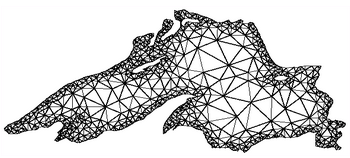
\includegraphics[width=\linewidth,keepaspectratio]{usMesh_wo_partitioning.png}
\caption{ Typical finite element mesh in 2 dimensional domain \label{usMesh_wo_partitioning}}
\endminipage\hfil
\minipage{0.1\textwidth}
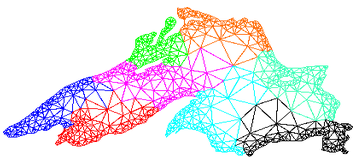
\includegraphics[width=\linewidth,keepaspectratio]{usMesh_w_partitioning.png}
\caption{ Partitioned mesh into eight sub domains \label{usMesh_w_partitioning}}
\endminipage\hfill
\end{figure}

There are two main approaches to perform partitioning\cite{Boman:2012:ZIP:2590399.2590404}. Those are, 
\begin{itemize}
 \item Space Filling Curve (SFC) based partitioning
 \item Graph based partitioning
\end{itemize}

%\begin{wraptable}{c}{3cm} % Left or right alignment is specified in the first bracket, the width of the table is in the second
\color{black}
\begin{multicols}{2}
\textbf{Graph Partitioning}
\begin{itemize}
 \item Widely used for static partitioning tasks.
 \item No geometric locality of objects preserved.
 \item No linear ordering of objects.
 \item Not incremental when mesh becomes finer.
\end{itemize}
\columnbreak
\textbf{SFC Partitioning}
\begin{itemize}
 \item Widely used for dynamic partitioning tasks.
 \item Geometric locality of objects preserved in partitioning.
 \item Linear ordering of objects may improve the cache performance.
 \item Easily incremental and adaptive approach.
\end{itemize}
\end{multicols}


%\end{wraptable}




%----------------------------------------------------------------------------------------
%	OBJECTIVES
%----------------------------------------------------------------------------------------

\color{ForestGreen}

\section*{Our Contributions}

\begin{enumerate}
\item We propose a new algorithm based on NCA to compute the Hilbert ordering, 9 times faster than the recursive approach.
\item Our NCA based algorithm is easily extensible to compute the ordering of any generic SFC (i.e. Morton, Peano etc.)
\item We empirically show that by introducing some flexibility(slack) to the load balancing, we can reduce the communication costs further, improving the efficiency of
overall computation. 
\end{enumerate}

%----------------------------------------------------------------------------------------
%	MATERIALS AND METHODS
%----------------------------------------------------------------------------------------
\color{DarkSlateGray} % DarkSlateGray color for the rest of the content
\section*{Methodology}

\subsection*{Space Filling Curves (SFC)}
SFC is a surjective mapping between the one dimensional space to higher dimensional space. Generally almost all the SFC adhere to the recursive nature in curve generation.Because of the recursive
nature SFCs have, most of the SFCs can be computed recursively.

Here are the images of Hilbert and Morton Space filling curves. 

\begin{figure}[H]
\centering
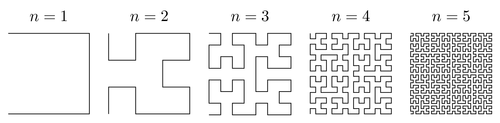
\includegraphics[height=40mm,keepaspectratio]{hilbertcurve.png}
\caption{ 2 dimensional Hilbert Curve with varying depth \label{hilbertcurve}}
\end{figure}

\begin{figure}[H]
\minipage{0.1\textwidth}
\centering
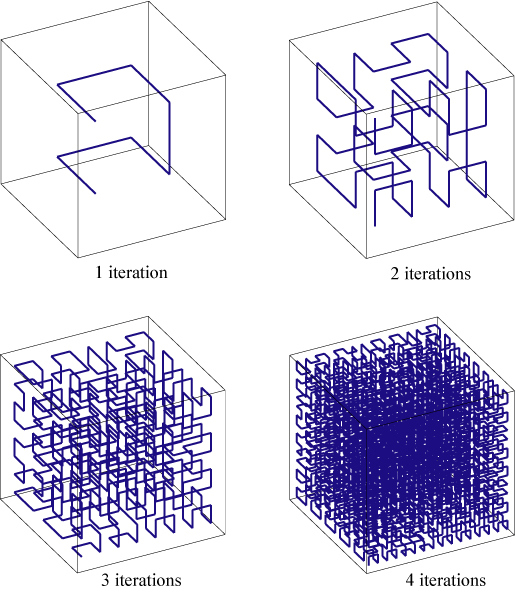
\includegraphics[width=0.8\linewidth,keepaspectratio]{hilbertcurve3d.jpg}
\caption{ 3 dimensional Hilbert Curve with varying depth \label{hilbertcurve3d}}
\endminipage\hfil
\minipage{0.1\textwidth}
\centering
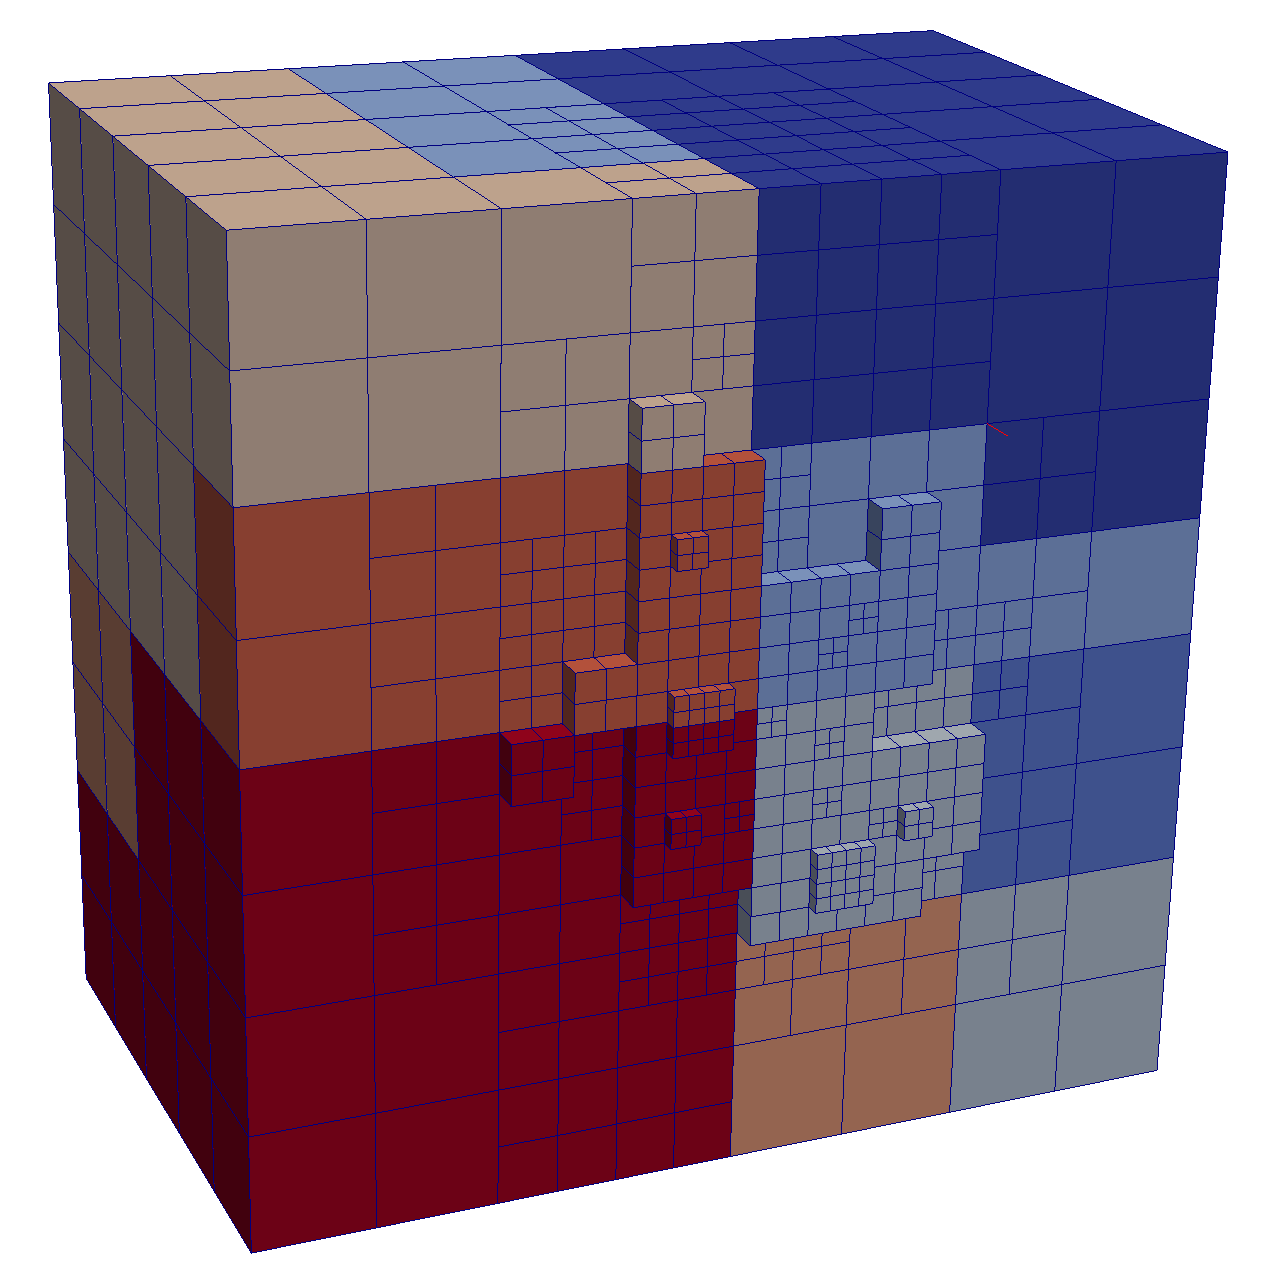
\includegraphics[width=0.8\linewidth,keepaspectratio]{morton.png}
\caption{ 2 dimensional Morton Curve with varying depth \label{morton}}
\endminipage\hfill
\end{figure}

%------------------------------------------------

\subsection*{New Nearest Common Ancestor (NCA) based Hilbert Ordering}

% \textcolor{blue}{Octree is a tree data structure which each internal node has exactly eight children.} Octrees are commonly used to represent the partitioning of 3 dimensional space by recursive sub division to eight
% octants. See Figure \ref{NCA} (2d scenario).

\textcolor{red}{The NCA of a two given octants (or coordinates)} (see Fig. \ref{NCA}), is the octant which encloses both given octants and the closest to the given two contants (or coordinates). \\
\color{orange}
The new NCA based Hilbert ordering computed as
follows. 
\begin{itemize}
 \item Compute the Nearest Common Ancestor(NCA) of the two octants.
 \item Traverse the octree from root to NCA once in order to compute the rotation pattern inside the considering NCA
 \item Use the rotation pattern inside the NCA to determine the relative ordering of the given octants.
\end{itemize}

\color{DarkSlateGray}
%\begin{wrapfigure}{R}{0.15\textwidth}
\subsection*{Improving the efficiency of Rotation Pattern Calculation}
We have improved the rotation pattern calculation for given NCA octant by using the following properties of the Hilbert curve.
\begin{itemize}
 \item If we fixed upon a initial Hilbert ordering \textit{\textcolor{red}{ Hilbert curve has 4 unique rotation patterns}} and \textit{\textcolor{red}{3D Hilbert curve has 24 unique rotation patterns}}.
 \item We store each rotation pattern and all it's children patterns in hard coded array which can be used to figure out the child rotation pattern for a given octant. The storage required to store the rotation patterns is fixed (\textit{\textcolor{blue}{In 2D we need $4\times4$  and in 3D we need $24\times8$}}) and independent from the Hilbert Curve order.
 \item By this approach we can compute the ordering between $P_1$ and $P_2$ by $O(Depth(NCA(P_1,P_1)))$
\end{itemize}

\begin{figure}[H]
\centering
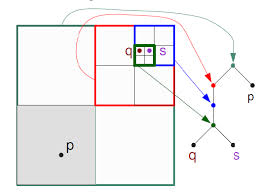
\includegraphics[width=0.1\textwidth,keepaspectratio]{nca.jpg}
\caption{Nearest Common Ancestor (NCA) of an octree (In this scenario, immediate parent node of nodes q and s is the NCA for nodes q and s. Relative ordering of q and s will be depend on the rotation pattern inside the NCA (See Fig. \ref{zcell} \& \ref{hilbertcell})) \label{NCA}} 
\end{figure}
%\end{wrapfigure}

\begin{multicols}{2}
\begin{figure}[H]
\centering
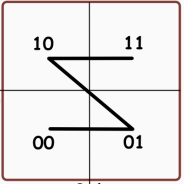
\includegraphics[width=0.5\columnwidth,keepaspectratio]{zcell.png}
\caption{Morton curve traversing pattern \label{zcell}}
\end{figure}
\columnbreak

\begin{figure}[H]
\centering
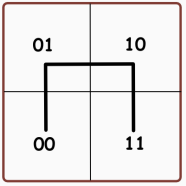
\includegraphics[width=0.5\columnwidth,keepaspectratio]{hilbertcell.png}
\caption{Hilbert curve traversing pattern \label{hilbertcell}}
\end{figure}
\end{multicols}
 




Even though there are multiple SFCs available, we mainly focus on the Morton and Hilbert curves and their ordering computations. To compare the NCA based ordering approach with other approaches we have
implemented both Hilbert and Morton as follows.
\color{olive}
\begin{itemize}
 \item Hilbert ordering baseline implementation (based on recursive approach)
 \item Morton ordering baseline implementation (based on non-recursive approach (i.e current implementation in dendro\cite{Sampath:2008:DPA:1413370.1413389}))
 \item Hilbert ordering NCA implementation (based on NCA approach)
 \item Morton ordering NCA implementation (based on NCA approach)
\end{itemize}

\color{DarkSlateGray}
\subsection*{Allowing Flexibility in Dynamic Load Balancing}

In this research we introduce some flexibility (slack) to the load balancing (i.e near uniform load balancing) in order to reduce the communication costs and reduce the overall execution time of the computation.
To demonstrate that we conduct two experiments.

\begin{itemize}
 \item \color{brown}Standard SFC based partition, where the work is uniform across all processes and compare the communication (using the surface area of the partition as a surrogate)
 \item \color{brown}A flexible SFC based partition, where we allow a small 'slack' (flexibility) in the amount of work that each process gets in order to reduce the communication costs. 
\end{itemize}


%----------------------------------------------------------------------------------------
%	RESULTS 
%----------------------------------------------------------------------------------------

\section*{Results}

Following figures show (See Fig.\ref{3d_NCA} \& \ref{2d_NCA}) the results of the four approaches that we implemented in order to compare the NCA based ordering Vs recursive based ordering.
By considering the mean execution time (ms) along the varying depth, we can conclude that the NCA based Hilbert ordering is 9 times faster than the traditional recursive based approach. If we consider the
NCA based Morton implementation mean execution time (ms) along the varying depth, we can see that it is 1.13 times slower than the Morton baseline implementation (implementation in dendro\cite{Sampath:2008:DPA:1413370.1413389}). 

% \setlength{\columnseprule}{0pt}
% \begin{multicols}{2}
% \begin{figure}[H]
% \centering
% \begin{tikzpicture}
% \pgfplotsset{height=7cm,compat=1.9}
% \begin{axis}[
% 	x tick label style={
% 		/pgf/number format/1000 sep=},
% 	ylabel=Execution Time (ms),
% 	enlargelimits=0.05,
% 	legend style={at={(0.5,-0.2)},
% 	anchor=north,legend columns=-1},
% 	ybar interval=0.7,
% ]
% 
% \addplot
% coordinates{
% (2,2113.2)
% (3,3548.5)
% (4,5568.55)
% (5,8076.45)
% (6,11155.1)
% (7,14914.1)
% (8,19654.2)
% (9,23992.8)
% (10,26824.8)
% };
% 
% \addplot 
% coordinates {
% (2,4794.05)
% (3,9315.4)
% (4,15656.7)
% (5,24192.2)
% (6,33925.6)
% (7,39182.8)
% (8,40351.1)
% (9,40485.9)
% (10,40510.8)};
% 
% 
% \legend{HilbertBL 2D, HilbertBL 3D}
% \end{axis}
% \end{tikzpicture}
% \caption{2d \& 3d ordering of Hilbert curve using recursive approach\label{recursive}}
% \end{figure}

% \hfill
% \columnbreak


% \end{multicols}


%\setlength{\columnseprule}{0pt}
% \begin{multicols}{2}
% \begin{figure}[H]
% \centering
% \begin{tikzpicture}
% \pgfplotsset{width=8cm,compat=1.9}
% \begin{axis}[
% 	x tick label style={
% 		/pgf/number format/1000 sep=},
% 	ylabel=Execution Time (ms),
% 	enlargelimits=0.05,
% 	legend style={at={(0.4,-0.2)},
% 	anchor=north,legend columns=-1},
% 	ybar interval=0.7,
% ]
% 
% \addplot %Hilbert Baseline 2D
% coordinates{
% (2,2113.2)
% (3,3548.5)
% (4,5568.55)
% (5,8076.45)
% (6,11155.1)
% (7,14914.1)
% (8,19654.2)
% (9,23992.8)
% (10,26824.8)
% };
% 
% \addplot % Hilbert NCA
% coordinates {
% (2,910.7)
% (3,1004.7)
% (4,1197.8)
% (5,1417.75)
% (6,1683.6)
% (7,1994.9)
% (8,2402.8)
% (9,2983.95)
% (10,3370.5)
% };
% 
% \addplot %Morton Baseline
% coordinates{
% (2,1058.45)
% (3,1068.2)
% (4,1060.8)
% (5,1083.6)
% (6,1135)
% (7,1196.8)
% (8,1284.6)
% (9,1443.55)
% (10,1543.65)
% };
% 
% \addplot %Morton NCA
% coordinates{
% 
% (2,836.55)
% (3,894.85)
% (4,955.7)
% (5,1038.6)
% (6,1141.75)
% (7,1256.65)
% (8,1410.8)
% (9,1654.6)
% (10,1864.9)
% 
% };
% 
% \legend{Hilbert BL,Hilbert NCA, Morton BL, Morton NCA}
% \end{axis}
% 
% 
% 
% \end{tikzpicture}
% \caption{2d ordering of points for Hilbert and Morton baseline, Hilbert and Morton NCA approaches.\label{2d_NCA}}
% \end{figure}
% \hfill
% 
% \columnbreak

\begin{figure}[H]
\centering
\begin{tikzpicture}
\pgfplotsset{width=8cm,compat=1.9}
\begin{axis}[
	x tick label style={
		/pgf/number format/1000 sep=},
        ylabel=Execution Time (ms),
	enlargelimits=0.05,
	legend style={at={(0.4,-0.2)},
	anchor=north,legend columns=-1},
	ybar interval=0.7,
	xbar bar width=0.1cm
	enlarge x limits=0.07	
]


% \addplot % Hilbert Baseline 3D
% coordinates {
% (2,4794.05)
% (3,9315.4)
% (4,15656.7)
% (5,24192.2)
% (6,33925.6)
% (7,39182.8)
% (8,40351.1)
% (9,40485.9)
% (10,40510.8)};
% 
% 
% \addplot % Hilbert NCA
% coordinates {
% (2,1088.75)
% (3,1425.8)
% (4,1912.6)
% (5,2576.95)
% (6,3627.5)
% (7,4263.65)
% (8,4444.95)
% (9,4515)
% (10,4575.8)
% };
% 
% \addplot %Morton Baseline
% coordinates{
% (2,1100.3)
% (3,1069.15)
% (4,1114.45)
% (5,1218.1)
% (6,1453.4)
% (7,1571.35)
% (8,1571.5)
% (9,1564.6)
% (10,1561.65)
% };
% 
% \addplot %Morton NCA
% coordinates{
% 
% (2,963.65)
% (3,1037.5)
% (4,1172.55)
% (5,1356.35)
% (6,1695.85)
% (7,1936.7)
% (8,2028.25)
% (9,2097.5)
% (10,2161.45)
% 
% };

\addplot % Hilbert Baseline 3D
coordinates {
(2,5494.05)
(4,17982)
(6,39330.2)
(8,46483.6)
(10,46684.9)
% (15,46578.8)
% (30,46803.8)
(12,10)
};


\addplot % Hilbert NCA
coordinates {
(2,2606.2)
(4,3655.95)
(6,4632.3)
(8,5103.65)
(10,5333.15)
% (15,5880.2)
% (30,7758.5)
(12,10)
};

\addplot %Morton Baseline
coordinates{
(2,2140.85)
(4,2562.7)
(6,2779.6)
(8,2990.65)
(10,2915.3)
% (15,2882.4)
% (30,2919.95)
(12,10)
};

\addplot %Morton NCA
coordinates{
(2,2001.9)
(4,2611.75)
(6,3052.65)
(8,3610.1)
(10,3771.6)
% (15,4324.25)
% (30,6488.5)
(12,10)

};



\legend{Hilbert BL,Hilbert NCA, Morton BL, Morton NCA}
\end{axis}
\end{tikzpicture}
\caption{3d ordering of points for Hilbert and Morton baseline, Hilbert and Morton NCA approaches.\label{3d_NCA}}
\end{figure}
% \hfill
% 
% \end{multicols}
% \setlength{\columnseprule}{2pt}

In the second experiment we allow some flexibility to the load, and observe how contour ratio (ratio between the surface area of the mesh that each node gets with some flexibility, Vs 0 flexibility case)
behaves with Hilbert and Morton ordering based partitioning. Our results show that (see Fig.\ref{flexibility}) by using the Hilbert ordering we can achieve low contour ratios compared with the Morton ordering which implies low
communication costs.We can conclude that by using Hilbert ordering with some flexibility we can reduce communication costs further compared to the Morton ordering (even with some flexibility).

\begin{figure}[H]
\centering
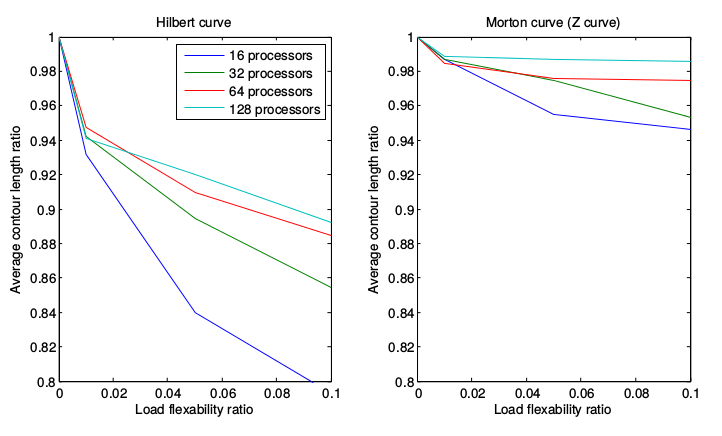
\includegraphics[height=7cm,keepaspectratio]{flexibility.png}
\caption{ Flexible partitioning results using Hilbert and Morton ordering \label{flexibility}}
\end{figure}




%----------------------------------------------------------------------------------------
%	CONCLUSIONS
%----------------------------------------------------------------------------------------

\color{SaddleBrown} % SaddleBrown color for the conclusions to make them stand out

\section*{Conclusions}

\begin{itemize}
\item Hilbert ordering is better than Morton ordering in terms of preserving the geometric locality of objects. 
\item We can conclude that the NCA based Hilbert ordering algorithm is 9 times faster than the traditional recursive approach for Hilbert ordering. 
%\item Our NCA based algorithm is easily extensible to compute the ordering of any generic SFC (i.e. Morton, Peano etc.)
\item Allowing some flexibility to the load at each node can reduce the communication further  (approximately in the range of 1.125-1.175 times), and reduce the overall computation time. 
\end{itemize}

\color{DarkSlateGray} % Set the color back to DarkSlateGray for the rest of the content

%----------------------------------------------------------------------------------------
%	FORTHCOMING RESEARCH
%----------------------------------------------------------------------------------------

%\section*{Forthcoming Research}

%Even though the current Hilbert ordering implementation is 


%----------------------------------------------------------------------------------------
%	REFERENCES
%----------------------------------------------------------------------------------------

\nocite{*} % Print all references regardless of whether they were cited in the poster or not
\bibliographystyle{plain} % Plain referencing style
\bibliography{hilbert} % Use the example bibliography file sample.bib

%----------------------------------------------------------------------------------------
%	ACKNOWLEDGEMENTS
%----------------------------------------------------------------------------------------

% \section*{Acknowledgements}
% 
% Etiam fermentum, arcu ut gravida fringilla, dolor arcu laoreet justo, ut imperdiet urna arcu a arcu. Donec nec ante a dui tempus consectetur. Cras nisi turpis, dapibus sit amet mattis sed, laoreet.

%----------------------------------------------------------------------------------------

\end{multicols}
\end{document}